\section{Sensitivity Grids}\label{sec: Sensitivity}
\subsection{The Remaining \ac{LWTA} Models - Channel-Out and \ac{SCO}}\label{appendix:Ensembles}
\begin{figure}[H]
    \makebox[\linewidth][c]{%
    \centering
    \begin{subfigure}{.5\textwidth}
        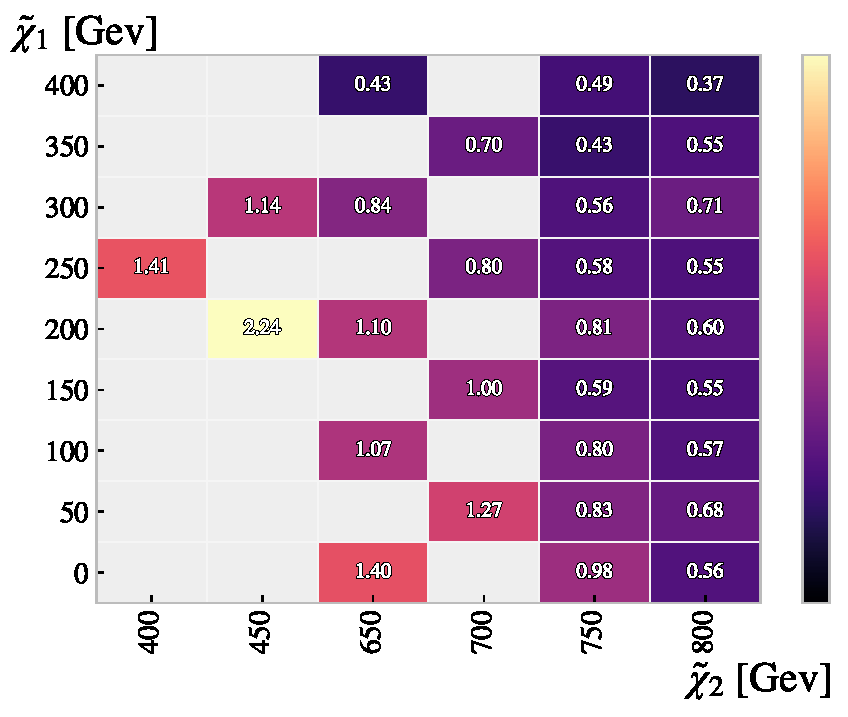
\includegraphics[width=\textwidth]{Figures/MLResults/NN/SUSY/Grid/StochChannelOutGridSig.pdf}
        \vspace{-1cm}
        \caption{}
        \label{fig:StochChannelOutGridSig}
    \end{subfigure}
    \begin{subfigure}{.5\textwidth}
        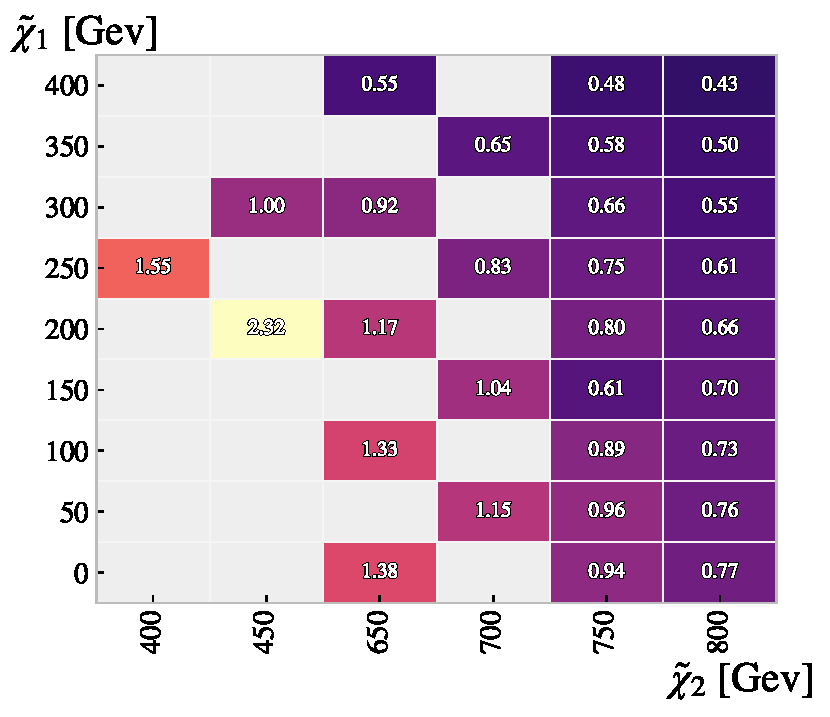
\includegraphics[width=\textwidth]{Figures/MLResults/NN/SUSY/Grid/ChannelOutGridSig.pdf}
        \vspace{-1cm}
        \caption{}
        \label{fig:ChannelOutGridSig}
    \end{subfigure}
    }
    \caption{A grid displaying the achieved significance on the original signal set, using the signal region 
    created by the \ac{SCO} \ref{fig:StochChannelOutGridSig} and a channel-out network \ref{fig:ChannelOutGridSig}.}
    \label{fig:SCOCO}
\end{figure}

\subsection{Results from the \ac{PCA}}\label{appendix:PCA}
\begin{figure}[H]
    \makebox[\linewidth][c]{%
    \centering
    \begin{subfigure}{.5\textwidth}
        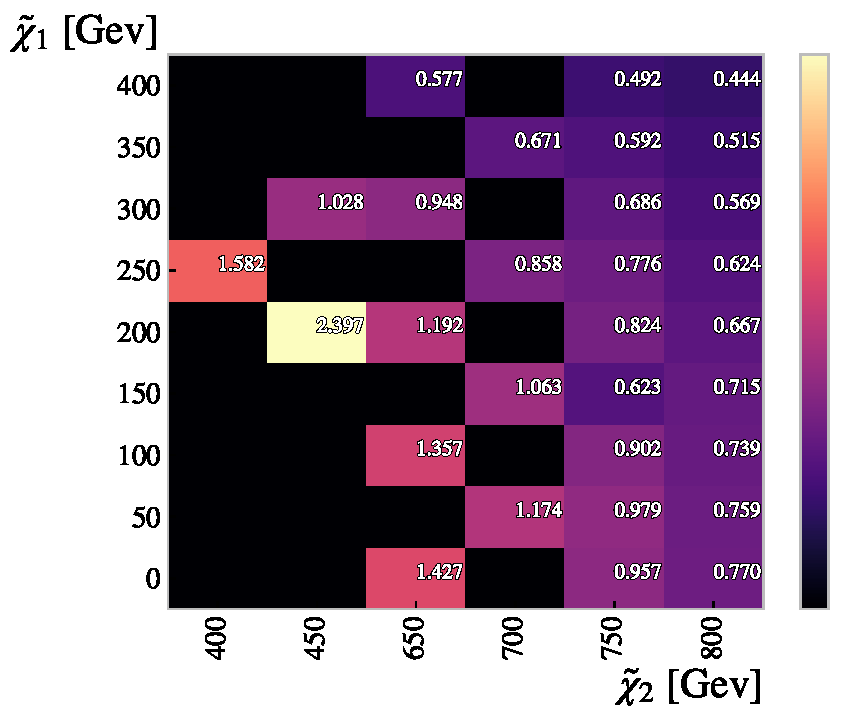
\includegraphics[width=\textwidth]{Figures/MLResults/NN/SUSY/Grid/NNPCAGridSig.pdf}
        \caption{}
        \label{fig:NNPCAGridSig}
    \end{subfigure}
    \begin{subfigure}{.5\textwidth}
        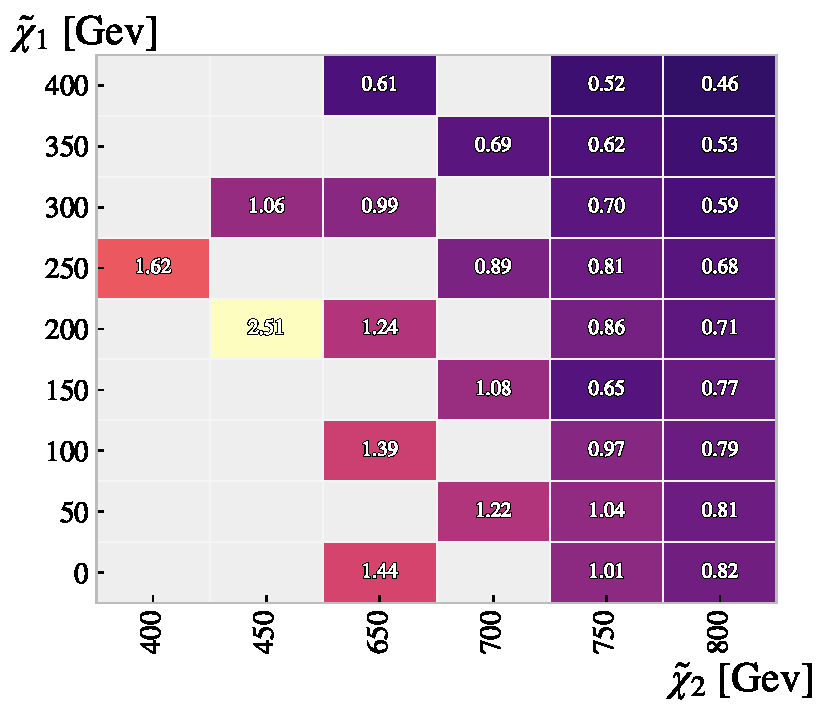
\includegraphics[width=\textwidth]{Figures/MLResults/NN/SUSY/Grid/MaxOutPCAGridSig.pdf}
        \caption{}
        \label{fig:MaxOutPCAGridSig}
    \end{subfigure}
    }
    \caption{A grid displaying the achieved significance on the original signal set, using the signal region 
    created by the \ac{NN} \ref{fig:NNPCAGridSig} and a maxout network \ref{fig:MaxOutPCAGridSig}. A \ac{PCA} 
    analysis has been applied to the data being utilized in this result.}
\end{figure}

\begin{figure}[H]
    \makebox[\linewidth][c]{%
    \centering
    \begin{subfigure}{.65\textwidth}
        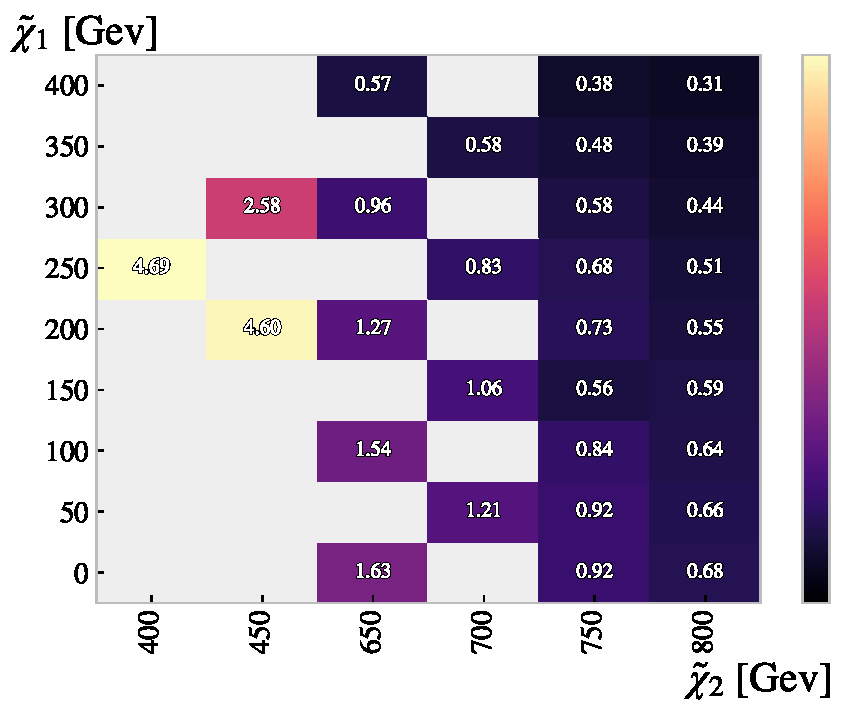
\includegraphics[width=\textwidth]{Figures/MLResults/NN/SUSY/Grid/PNNPCAGridSig.pdf}
    \end{subfigure}
    }
    \caption{A grid displaying the achieved significance on the original signal set, using the signal region 
    created by the \ac{PNN} network. A \ac{PCA} analysis has been applied to the data being utilized in this result.}
    \label{fig:PNNPCAGridSig}
\end{figure}

\begin{figure}[H]
    \makebox[\linewidth][c]{%
    \centering
    \begin{subfigure}{.65\textwidth}
        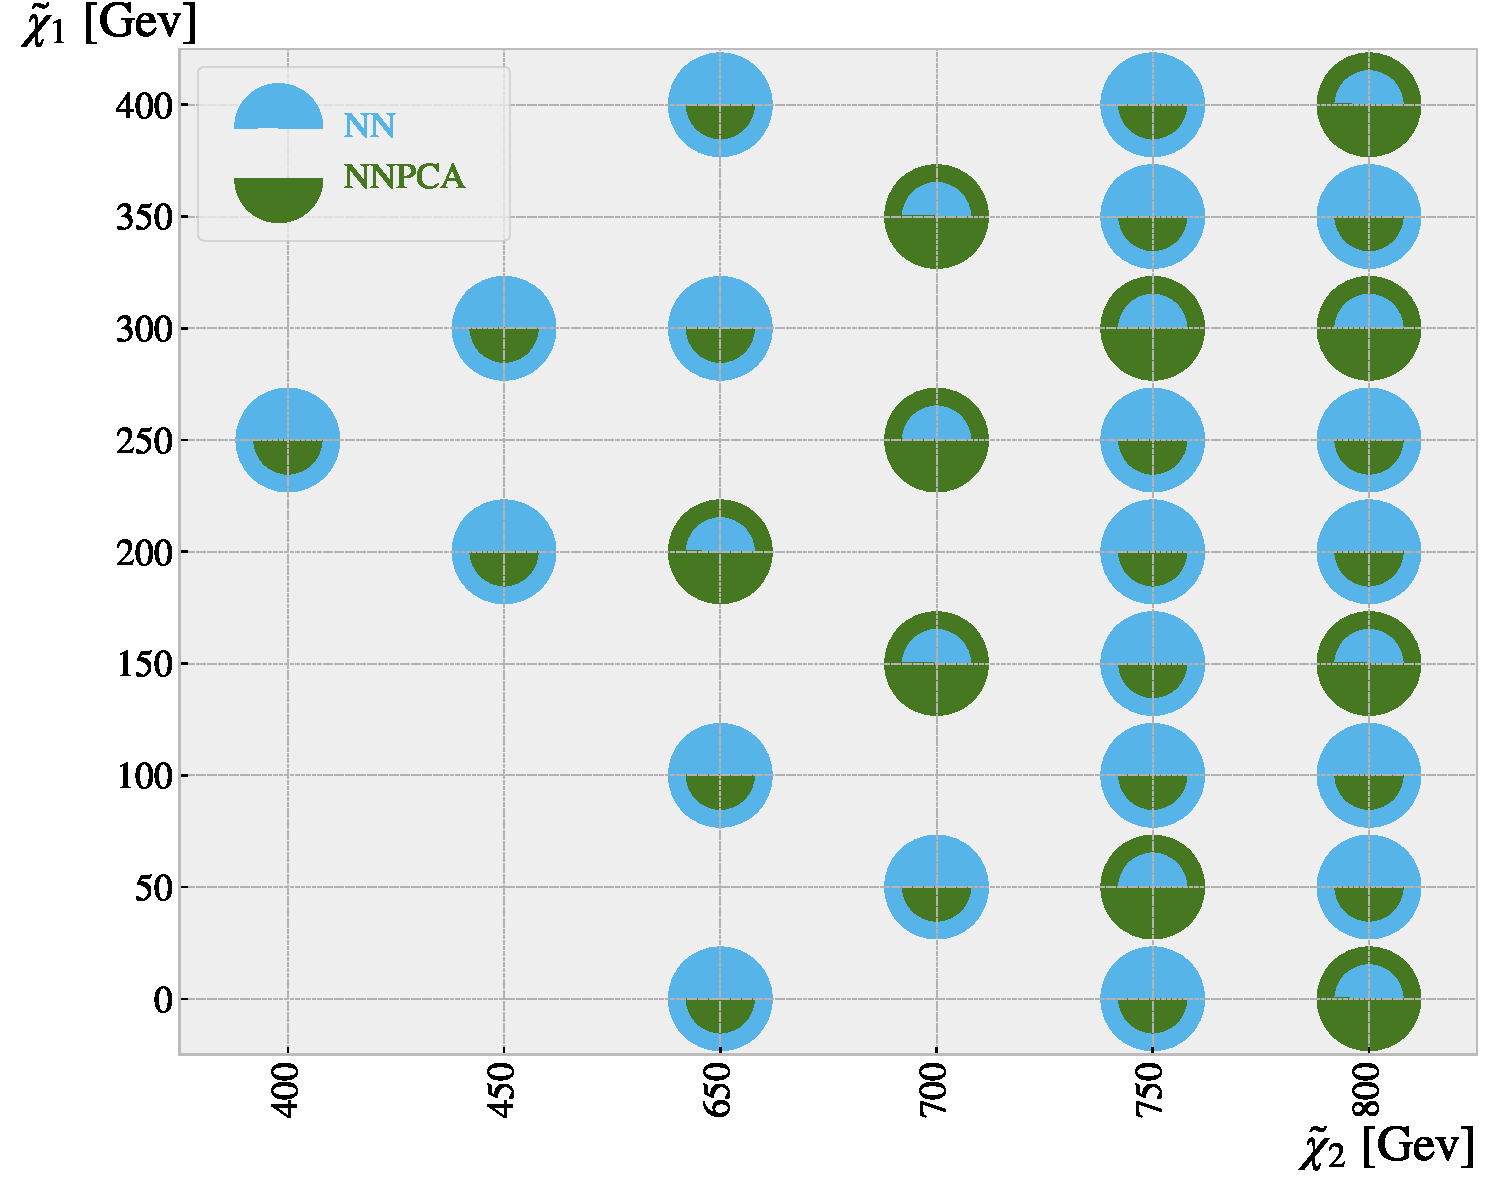
\includegraphics[width=\textwidth]{Figures/MLResults/NN/SUSY/Comparison/NNPCANetworkComp.pdf}
    \end{subfigure}
    }
    \caption{A grid displaying the achieved significance on the original signal set, using the signal region 
    created by the \ac{NN} network. A \ac{PCA} analysis has been applied to the data being utilized in this result.}
    \label{fig:NNPCAComp}
\end{figure}
\newpage